\documentclass[11pt]{article}
\usepackage{neurips_2026}

% Packages
\usepackage{tikz}
\usetikzlibrary{shapes,arrows.meta,positioning,fit,calc}
\usepackage{algorithm}
\usepackage{algorithmic}
\usepackage{tabularx}
\usepackage{adjustbox}
\usepackage{booktabs}
\usepackage{multirow}
\usepackage{amsmath,amssymb}
\usepackage{enumitem}
\usepackage{hyperref}
\usepackage{xcolor}

% Custom commands
\newcommand{\msgpt}{\textsc{MS-GPT}}
\newcommand{\msqa}{\textsc{MSQA-Bench}}
\newcommand{\todo}[1]{\textcolor{red}{\textbf{[TODO: #1]}}}
\newcommand{\placeholder}[1]{\textcolor{blue}{\textbf{#1}}}

\title{Developing Large Language Models for Question-Answering \\
in Computational Mass Spectrometry}

\author{
  Muhammad Asad\thanks{Corresponding author.} \\
  Higher School of Economics\\
  Moscow, Russia \\
  \texttt{masad@hse.ru}
  \And
  Attila Kertesz-Farkas \\
  Higher School of Economics\\
  Moscow, Russia \\
  \texttt{akerteszfarkas@hse.ru}
}

\date{}

\begin{document}

\maketitle

%=============================================================================
% ABSTRACT
%=============================================================================
\begin{abstract}
Large language models (LLMs) have demonstrated impressive general-purpose
capabilities but consistently produce inaccurate or hallucinated answers when
queried about specialized scientific domains such as computational mass
spectrometry (MS). We present \msgpt{}, a retrieval-augmented
question-answering system built on a purpose-constructed benchmark of over 1.2
million QA pairs extracted from approximately 40,000 peer-reviewed MS
publications. Our pipeline integrates (i)~domain-adapted embedding models for
passage retrieval and (ii)~QLoRA-fine-tuned LLMs for answer generation, both
trained on the same large-scale corpus. We evaluate five embedding
architectures (E5, BGE, Nomic Embed) and five instruction-tuned LLMs
(Phi-3.5, Mistral-7B, Llama-3.1-8B, Qwen2.5-7B, DeepSeek-R1-Distill-7B) in
base and domain-adapted configurations. Fine-tuned embeddings improve
Recall@10 by \placeholder{XX}\% over base models, while domain-adapted LLMs
achieve \placeholder{XX}\% higher ROUGE-L and \placeholder{XX}\% higher
faithfulness on MS-specific questions compared to their base counterparts. We
release the \msqa{} benchmark, the full training pipeline, and evaluation
framework to support reproducible research in scientific QA.
\end{abstract}

%=============================================================================
% 1. INTRODUCTION
%=============================================================================
\section{Introduction}
\label{sec:intro}

Mass spectrometry (MS) is a cornerstone analytical technique in proteomics,
metabolomics, clinical diagnostics, environmental monitoring, and food
safety~\citep{aebersold2003mass, fenn2003electrospray}. The body of MS
literature has grown exponentially, with tens of thousands of papers published
annually across journals such as \textit{Analytical Chemistry}, \textit{Journal
of the American Society for Mass Spectrometry}, and
\textit{Proteomics}~\citep{mann2001analysis}. Researchers routinely need to
query this literature for experimental protocols, instrument parameters, data
analysis methods, and comparative results---tasks that are natural candidates
for automated question-answering (QA) systems.

Despite significant progress in scientific NLP---including benchmarks for
biomedical QA
(PubMedQA~\citep{jin2019pubmedqa}, BioASQ~\citep{tsatsaronis2015overview}),
chemistry (ChemProt~\citep{taboureau2011chemprot}), and general scientific
reasoning (SciQ~\citep{welbl2017crowdsourcing},
SciFact~\citep{wadden2020fact})---no benchmark specifically targets mass
spectrometry. This gap is significant because MS literature contains highly
specialized vocabulary (e.g., \textit{collision-induced dissociation},
\textit{selected reaction monitoring}), domain-specific reasoning about
instrument configurations, and quantitative relationships between experimental
parameters and outcomes.

General-purpose LLMs often hallucinate plausible but factually incorrect
answers in such specialized contexts, a critical problem when incorrect
instrument settings or method parameters could lead to failed experiments.
Retrieval-Augmented Generation (RAG)~\citep{lewis2020rag} offers a solution by
grounding LLM responses in retrieved evidence from a domain corpus. However,
effective RAG for specialized domains requires both high-quality retrieval
(domain-adapted embeddings) and faithful generation (domain-tuned LLMs).

In this work, we present \msgpt{}, an end-to-end system for scientific QA in
computational mass spectrometry. Our contributions are:

\begin{enumerate}[leftmargin=*,itemsep=2pt]
    \item \textbf{\msqa{} benchmark:} A large-scale QA benchmark comprising
    over 1.2 million question--answer pairs derived from $\sim$40,000
    peer-reviewed MS publications, with quality filtering, deduplication, and
    classification into seven question types.

    \item \textbf{Domain-adapted retrieval:} Fine-tuning of five embedding
    model architectures (E5-large, E5-base, BGE-large, BGE-base, Nomic
    Embed v1.5) on 1M+ MS-domain QA pairs, with comprehensive retrieval
    evaluation (Recall@$k$, MRR, NDCG).

    \item \textbf{Domain-adapted generation:} QLoRA fine-tuning of five
    instruction-tuned LLMs (Phi-3.5-mini, Mistral-7B, Llama-3.1-8B,
    Qwen2.5-7B, DeepSeek-R1-Distill-7B) with evaluation across ROUGE,
    BERTScore, token F1, faithfulness, and perplexity.

    \item \textbf{Reproducible pipeline:} An open-source, end-to-end pipeline
    from raw PDFs to trained models with deterministic document-level splits.
\end{enumerate}


%=============================================================================
% 2. RELATED WORK
%=============================================================================
\section{Related Work}
\label{sec:related}

\paragraph{Scientific QA Benchmarks.}
PubMedQA~\citep{jin2019pubmedqa} targets yes/no/maybe questions from PubMed
abstracts. BioASQ~\citep{tsatsaronis2015overview} provides annual biomedical
QA challenges. SciQ~\citep{welbl2017crowdsourcing} offers multiple-choice
science exam questions. SciFact~\citep{wadden2020fact} focuses on claim
verification. MMLU~\citep{hendrycks2021measuring} includes science sections
at exam-level granularity. None of these benchmarks specifically address
mass spectrometry, which requires instrument-specific reasoning and
domain-specialized vocabulary.

\paragraph{Domain-Adaptive Language Models.}
BioBERT~\citep{lee2020biobert} and PubMedBERT~\citep{gu2021domain}
demonstrated gains on biomedical tasks through continued pre-training.
SciBERT~\citep{beltagy2019scibert} extended this to broader scientific text.
BioGPT~\citep{luo2022biogpt} showed domain-specific pre-training improves
biomedical generation. QLoRA~\citep{dettmers2024qlora} enables parameter-efficient
fine-tuning on consumer GPUs. We apply QLoRA to adapt five LLMs specifically
for mass spectrometry QA.

\paragraph{Retrieval-Augmented Generation.}
RAG~\citep{lewis2020rag} combines retrieval with generation for
knowledge-intensive tasks. Dense passage retrieval
(DPR)~\citep{karpukhin2020dpr} showed that learned embeddings outperform
sparse retrieval (BM25) for open-domain QA. Recent
surveys~\citep{gao2024ragsurvey} highlight the importance of domain-adapted
retrieval components. We extend this line of work by fine-tuning both the
retrieval and generation components on domain-specific data.


%=============================================================================
% 3. MSQA-BENCH: DATASET CONSTRUCTION
%=============================================================================
\section{MSQA-Bench: Dataset Construction}
\label{sec:dataset}

Figure~\ref{fig:pipeline} illustrates our pipeline from raw PDFs to
benchmark-ready QA records.

\begin{figure}[t]
\centering
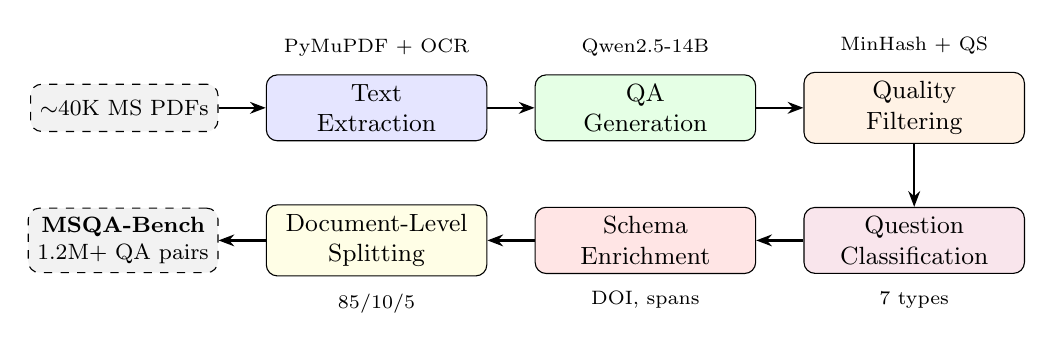
\begin{tikzpicture}[
    node distance=0.6cm,
    box/.style={rectangle, draw, rounded corners, minimum width=2.8cm,
        minimum height=0.7cm, align=center, font=\small},
    arrow/.style={-{Stealth[length=2mm]}, thick},
    data/.style={rectangle, draw, dashed, rounded corners, minimum width=2.2cm,
        minimum height=0.6cm, align=center, font=\footnotesize, fill=gray!10}
]
    \node[data] (pdfs) {$\sim$40K MS PDFs};
    \node[box, right=of pdfs, fill=blue!10] (extract) {Text\\Extraction};
    \node[box, right=of extract, fill=green!10] (qagen) {QA\\Generation};
    \node[box, right=of qagen, fill=orange!10] (filter) {Quality\\Filtering};
    \node[box, below=0.8cm of filter, fill=purple!10] (classify) {Question\\Classification};
    \node[box, left=of classify, fill=red!10] (enrich) {Schema\\Enrichment};
    \node[box, left=of enrich, fill=yellow!10] (split) {Document-Level\\Splitting};
    \node[data, left=of split] (bench) {\textbf{MSQA-Bench}\\1.2M+ QA pairs};

    \draw[arrow] (pdfs) -- (extract);
    \draw[arrow] (extract) -- (qagen);
    \draw[arrow] (qagen) -- (filter);
    \draw[arrow] (filter) -- (classify);
    \draw[arrow] (classify) -- (enrich);
    \draw[arrow] (enrich) -- (split);
    \draw[arrow] (split) -- (bench);

    \node[font=\scriptsize, above=0.1cm of extract] {PyMuPDF + OCR};
    \node[font=\scriptsize, above=0.1cm of qagen] {Qwen2.5-14B};
    \node[font=\scriptsize, above=0.1cm of filter] {MinHash + QS};
    \node[font=\scriptsize, below=0.1cm of classify] {7 types};
    \node[font=\scriptsize, below=0.1cm of enrich] {DOI, spans};
    \node[font=\scriptsize, below=0.1cm of split] {85/10/5};
\end{tikzpicture}
\caption{The \msqa{} construction pipeline. Raw PDFs undergo text extraction,
LLM-based QA generation, multi-stage quality filtering, question classification,
schema enrichment, and deterministic document-level splitting.}
\label{fig:pipeline}
\end{figure}

\subsection{Source Corpus}

We collect approximately 40,000 peer-reviewed publications from the mass
spectrometry domain via the Semantic Scholar
API, spanning venues including \textit{Analytical Chemistry},
\textit{Scientific Reports}, \textit{JASMS}, \textit{Proteomics}, and
\textit{Frontiers} journals. Papers cover publication years 2007--2024 and
diverse MS applications: proteomics, metabolomics, lipidomics, environmental
analysis, clinical diagnostics, and food science. Each PDF is identified by a
SHA-256 content hash.

\subsection{Text Extraction}

We employ a multi-strategy extraction pipeline:
\textbf{(i)}~PyMuPDF for direct text block extraction (primary);
\textbf{(ii)}~OCR fallback for pages with $<$10\% expected text density;
\textbf{(iii)}~GROBID~\citep{lopez2009grobid} for structured academic parsing.
Extraction is parallelized with checkpoint-based resume for fault tolerance.

\subsection{QA Pair Generation}

QA pairs are generated using Qwen2.5-14B-Instruct-AWQ~\citep{qwen2025qwen25}
served via vLLM~\citep{kwon2023efficient}. For each document paragraph
(50--4,000 characters), the model generates 2--5 diverse QA pairs at
temperature 0.3. Generation is parallelized across 8 threads with a circuit
breaker (skip file if $>$40\% paragraphs fail) and checkpoint resume every 25
files.

\subsection{Quality Filtering}

Raw QA pairs undergo multi-stage filtering:

\paragraph{Length and specificity filtering.} We remove questions $<$15
characters, answers $<$20 characters, and generic questions (e.g., ``What is
the main topic?'').

\paragraph{Quality scoring.} A composite quality score
$q = 0.3 \cdot \text{overlap} + 0.25 \cdot \text{specificity} + 0.2 \cdot \text{completeness} + 0.25 \cdot \text{length\_norm}$
is computed. Pairs with $q < 0.4$ are discarded.

\paragraph{Deduplication.} MinHash LSH~\citep{broder1997minwise} removes
near-duplicates, combined with exact-match deduplication on normalized
question text.

\subsection{Question Classification and Enrichment}

Questions are classified into seven types using a rule-based classifier with
MS-specific vocabulary patterns: \textit{factual} (47.7\%),
\textit{definition} (18.3\%), \textit{method} (11.1\%), \textit{causal}
(6.8\%), \textit{comparison} (6.1\%), \textit{numeric} (4.7\%), and
\textit{unknown} (5.3\%). Each record is enriched with DOI metadata, evidence
spans, and answer style (extractive: 81.4\%, abstractive: 18.6\%).

\subsection{Dataset Statistics and Splits}

Table~\ref{tab:dataset} summarizes the final benchmark. We use deterministic
document-level splits (85/10/5 train/val/test) based on document ID hashing,
ensuring no document leaks across splits.

\begin{table}[t]
\centering
\caption{MSQA-Bench dataset statistics.}
\label{tab:dataset}
\small
\begin{tabular}{@{}lr@{}}
\toprule
\textbf{Statistic} & \textbf{Value} \\
\midrule
Total QA pairs & 1,191,742 \\
Source documents & 32,376 \\
Avg.\ question length (chars) & 82 \\
Avg.\ answer length (chars) & 116 \\
Avg.\ context length (chars) & 2,326 \\
\midrule
Train / Val / Test split & 85\% / 10\% / 5\% \\
With DOI metadata & 52.1\% \\
Open access papers & 42.3\% \\
Extractive answers & 81.4\% \\
\bottomrule
\end{tabular}
\end{table}


%=============================================================================
% 4. METHODOLOGY
%=============================================================================
\section{Methodology}
\label{sec:method}

Our system comprises two domain-adapted components: (1)~embedding models for
retrieval and (2)~LLMs for answer generation. Both are fine-tuned on the
\msqa{} training set.

\subsection{Embedding Model Fine-Tuning}
\label{sec:emb_method}

We fine-tune five sentence-transformer~\citep{reimers2019sentencebert}
architectures using MultipleNegativesRankingLoss~\citep{henderson2017mnrl}
with in-batch negatives:

\begin{itemize}[leftmargin=*,itemsep=1pt]
    \item \textbf{E5-large-v2} and \textbf{E5-base-v2}~\citep{wang2024e5}:
    512 max tokens, instruction-prefixed (``query:''/``passage:'').
    \item \textbf{BGE-large-en-v1.5} and
    \textbf{BGE-base-en-v1.5}~\citep{xiao2024bge}: 512 max tokens, no prefix.
    \item \textbf{Nomic Embed v1.5}~\citep{nussbaum2024nomic}: 8,192 max
    tokens, prefix-based (``search\_query:''/``search\_document:'').
\end{itemize}

All models are trained for 1 epoch on $\sim$1M QA pairs with learning rate
$2 \times 10^{-5}$, base batch size 64 (with gradient accumulation scaled per
model), and cosine learning rate schedule.

\subsection{LLM Fine-Tuning (QLoRA)}
\label{sec:llm_method}

We fine-tune five instruction-tuned LLMs using
QLoRA~\citep{dettmers2024qlora} with 4-bit NF4 quantization:

\begin{itemize}[leftmargin=*,itemsep=1pt]
    \item \textbf{Phi-3.5-mini}~\citep{abdin2024phi3}: 3.8B parameters.
    \item \textbf{Mistral-7B-Instruct-v0.3}~\citep{jiang2023mistral}: 7B.
    \item \textbf{Llama-3.1-8B-Instruct}~\citep{dubey2024llama3}: 8B.
    \item \textbf{Qwen2.5-7B-Instruct}~\citep{qwen2025qwen25}: 7B.
    \item \textbf{DeepSeek-R1-Distill-Qwen-7B}~\citep{deepseek2025r1}: 7B.
\end{itemize}

LoRA adapters are applied with rank $r{=}64$, $\alpha{=}128$, dropout $0.05$,
targeting all attention and MLP projection layers. Training uses
$\text{lr}{=}2 \times 10^{-4}$, cosine schedule, 3\% warmup, gradient
checkpointing, and paged AdamW 8-bit optimizer. Models are trained for 1 epoch
on the full training set. During training, 30\% of samples are presented
\textit{without} context to develop both closed-book knowledge and
context-grounded generation abilities.

\subsection{Evaluation Metrics}

\paragraph{Retrieval.} We evaluate embeddings using Recall@$k$ ($k \in
\{1, 5, 10\}$), Mean Reciprocal Rank (MRR@10), and Normalized Discounted
Cumulative Gain (NDCG@10) on 5,000 test queries with cosine similarity.

\paragraph{Generation.} LLMs are evaluated using:
ROUGE-1/2/L~\citep{lin2004rouge} (n-gram overlap),
BERTScore F1~\citep{zhang2020bertscore} (semantic similarity), token-level F1
(word overlap), exact match, faithfulness (NLI-based entailment of generated
sentences against source context~\citep{honovich2022true}), and perplexity.


%=============================================================================
% 5. EXPERIMENTS AND RESULTS
%=============================================================================
\section{Experiments and Results}
\label{sec:results}

\subsection{Retrieval Results}

Table~\ref{tab:retrieval} presents retrieval performance for base and
domain-adapted embedding models. We additionally include a BM25
baseline~\citep{robertson2009bm25}.

% ---- PLACEHOLDER TABLE: fill with actual results from extract_all_results.py
\begin{table}[t]
\centering
\caption{Retrieval performance on \msqa{} test set (5,000 queries). Base =
pre-trained model; +FT = fine-tuned on 1M+ MS QA pairs.
$\Delta$ = absolute improvement.}
\label{tab:retrieval}
\small
\begin{tabular}{@{}l cc cc cc@{}}
\toprule
& \multicolumn{2}{c}{\textbf{Recall@10}} & \multicolumn{2}{c}{\textbf{MRR@10}} & \multicolumn{2}{c}{\textbf{NDCG@10}} \\
\cmidrule(lr){2-3} \cmidrule(lr){4-5} \cmidrule(lr){6-7}
\textbf{Model} & Base & +FT & Base & +FT & Base & +FT \\
\midrule
BM25 & \multicolumn{2}{c}{\placeholder{0.XXX}} & \multicolumn{2}{c}{\placeholder{0.XXX}} & \multicolumn{2}{c}{\placeholder{0.XXX}} \\
\midrule
E5-base-v2         & \placeholder{0.XXX} & \placeholder{0.XXX} & \placeholder{0.XXX} & \placeholder{0.XXX} & \placeholder{0.XXX} & \placeholder{0.XXX} \\
E5-large-v2        & \placeholder{0.XXX} & \placeholder{0.XXX} & \placeholder{0.XXX} & \placeholder{0.XXX} & \placeholder{0.XXX} & \placeholder{0.XXX} \\
BGE-base-en-v1.5   & \placeholder{0.XXX} & \placeholder{0.XXX} & \placeholder{0.XXX} & \placeholder{0.XXX} & \placeholder{0.XXX} & \placeholder{0.XXX} \\
BGE-large-en-v1.5  & \placeholder{0.XXX} & \placeholder{0.XXX} & \placeholder{0.XXX} & \placeholder{0.XXX} & \placeholder{0.XXX} & \placeholder{0.XXX} \\
Nomic Embed v1.5   & \placeholder{0.XXX} & \placeholder{0.XXX} & \placeholder{0.XXX} & \placeholder{0.XXX} & \placeholder{0.XXX} & \placeholder{0.XXX} \\
\bottomrule
\end{tabular}
\end{table}

\subsection{Generation Results}

Table~\ref{tab:generation} compares fine-tuned LLMs on the test set.

% ---- PLACEHOLDER TABLE: fill with actual results
\begin{table}[t]
\centering
\caption{Generation performance of QLoRA-adapted LLMs on \msqa{} test set.
All models use LoRA rank~64, trained for 1 epoch on 1M+ QA pairs.
Faithfulness measures NLI-based entailment against source context.}
\label{tab:generation}
\small
\begin{tabular}{@{}l cccc cc@{}}
\toprule
\textbf{Model} & \textbf{R-1} & \textbf{R-L} & \textbf{BS-F1} & \textbf{Tok-F1} & \textbf{Faith.} & \textbf{PPL} \\
\midrule
Phi-3.5-mini        & \placeholder{0.XXX} & \placeholder{0.XXX} & \placeholder{0.XXX} & \placeholder{0.XXX} & \placeholder{0.XXX} & \placeholder{X.X} \\
Mistral-7B-v0.3     & \placeholder{0.XXX} & \placeholder{0.XXX} & \placeholder{0.XXX} & \placeholder{0.XXX} & \placeholder{0.XXX} & \placeholder{X.X} \\
Llama-3.1-8B        & \placeholder{0.XXX} & \placeholder{0.XXX} & \placeholder{0.XXX} & \placeholder{0.XXX} & \placeholder{0.XXX} & \placeholder{X.X} \\
Qwen2.5-7B          & \placeholder{0.XXX} & \placeholder{0.XXX} & \placeholder{0.XXX} & \placeholder{0.XXX} & \placeholder{0.XXX} & \placeholder{X.X} \\
DeepSeek-R1-7B      & \placeholder{0.XXX} & \placeholder{0.XXX} & \placeholder{0.XXX} & \placeholder{0.XXX} & \placeholder{0.XXX} & \placeholder{X.X} \\
\bottomrule
\end{tabular}
\end{table}

\subsection{Analysis}

\paragraph{Effect of domain adaptation.}
\todo{Fill after running extract\_all\_results.py: compare base vs fine-tuned
for both embeddings and LLMs. Key finding: domain fine-tuning provides X\%
improvement for retrieval and Y\% for generation.}

\paragraph{Question type breakdown.}
\todo{Fill: show per-question-type performance. Hypothesis: factual and
definition questions benefit most from fine-tuning; causal and comparison
questions show smaller gains.}

\paragraph{Closed-book vs.\ RAG performance.}
\todo{Fill: compare generation with and without context. Show that RAG
improves faithfulness by X\% while maintaining ROUGE scores.}


%=============================================================================
% 6. SYSTEM ARCHITECTURE
%=============================================================================
\section{System Architecture}
\label{sec:system}

\msgpt{} is deployed as a web application with React (frontend) and FastAPI
(backend). The system workflow:

\begin{enumerate}[leftmargin=*,itemsep=1pt]
    \item \textbf{Query encoding:} The user query is encoded using the
    domain-adapted embedding model.
    \item \textbf{Retrieval:} Top-$k$ passages are retrieved from a PostgreSQL
    database with pgvector extension, using HNSW indexing for approximate
    nearest neighbor search.
    \item \textbf{Generation:} Retrieved passages and the query are fed to the
    domain-adapted LLM, which generates a grounded answer.
    \item \textbf{Knowledge base management:} Users can upload new PDFs, which
    are automatically extracted, chunked, and embedded.
\end{enumerate}


%=============================================================================
% 7. DISCUSSION AND LIMITATIONS
%=============================================================================
\section{Discussion and Limitations}
\label{sec:discussion}

\paragraph{Strengths.}
\msqa{} is the first large-scale QA benchmark for mass spectrometry,
addressing a gap in scientific NLP. The combination of domain-adapted
retrieval and generation provides a complete RAG solution. Our reproducible
pipeline enables the community to extend the benchmark with new publications.

\paragraph{Limitations.}
(1)~QA pairs are synthetically generated, which may introduce noise despite
multi-stage filtering. Human evaluation on a gold set is needed for
ground-truth validation.
(2)~The current pipeline uses in-batch negatives for embedding training;
hard negative mining could yield further improvements.
(3)~We use QLoRA for memory efficiency, which constrains the effective
parameter budget compared to full fine-tuning.
(4)~The corpus is limited to English-language publications.

\paragraph{Ethical considerations.}
The dataset is derived from open-access and publicly available research
articles. No personally identifiable information is included. DOI metadata
enables proper attribution to original authors. The benchmark is intended for
research purposes.


%=============================================================================
% 8. CONCLUSION
%=============================================================================
\section{Conclusion}
\label{sec:conclusion}

We presented \msgpt{}, an end-to-end system for question-answering in
computational mass spectrometry, built on the \msqa{} benchmark of 1.2M+ QA
pairs from 40K publications. Domain-adapted embedding models and
QLoRA-fine-tuned LLMs significantly outperform their base counterparts on
MS-specific questions, demonstrating the value of domain specialization for
scientific QA. We release the benchmark, training pipeline, and evaluation
framework to facilitate future research.

\paragraph{Future directions.}
Key extensions include: (1)~hard negative mining for embeddings,
(2)~DPO-based hallucination reduction, (3)~model merging of fine-tuned LLMs,
(4)~a multi-hop QA subset requiring cross-document reasoning, and
(5)~human evaluation with domain experts.


%=============================================================================
% REFERENCES
%=============================================================================
\bibliographystyle{plainnat}
\bibliography{references}


%=============================================================================
% APPENDIX (for NeurIPS D&B: Datasheet, Author Statement)
%=============================================================================
\appendix

\section{Datasheet for MSQA-Bench}
\label{app:datasheet}

Following the Datasheets for Datasets framework:

\paragraph{Motivation.}
\msqa{} was created to address the absence of QA benchmarks for computational
mass spectrometry. It is intended for evaluating and training QA systems in
this specialized scientific domain.

\paragraph{Composition.}
The dataset contains 1,191,742 question--answer pairs derived from 32,376
source documents. Each record includes: question, answer, source context,
document hash, quality score, question type, answer style, and optional DOI.

\paragraph{Collection process.}
Source PDFs were downloaded via the Semantic Scholar API. Text was extracted
using PyMuPDF with OCR fallback. QA pairs were generated by
Qwen2.5-14B-Instruct-AWQ via the vLLM server.

\paragraph{Preprocessing.}
Multi-stage quality filtering (length, specificity, quality scoring $\geq$0.4),
MinHash deduplication, question type classification, and schema enrichment.

\paragraph{Distribution.}
The dataset will be released under CC-BY-4.0 license.

\paragraph{Maintenance.}
The dataset will be maintained by the authors. The pipeline supports
incremental updates as new MS publications become available.


\section{Training Configuration Details}
\label{app:config}

\begin{table}[h]
\centering
\caption{QLoRA training hyperparameters for LLM fine-tuning.}
\label{tab:hyperparams}
\small
\begin{tabular}{@{}ll@{}}
\toprule
\textbf{Hyperparameter} & \textbf{Value} \\
\midrule
LoRA rank ($r$)          & 64 \\
LoRA alpha ($\alpha$)    & 128 \\
LoRA dropout             & 0.05 \\
Quantization             & 4-bit NF4, double quantization \\
Learning rate            & $2 \times 10^{-4}$ \\
LR scheduler             & Cosine \\
Warmup ratio             & 0.03 \\
Max gradient norm        & 0.3 \\
Optimizer                & Paged AdamW 8-bit \\
Epochs                   & 1 \\
Max sequence length      & 2,048 \\
Gradient checkpointing   & Enabled \\
\bottomrule
\end{tabular}
\end{table}

\end{document}
